\documentclass{standalone}
\usepackage{tikz}
\usetikzlibrary{patterns, positioning}

\begin{document}
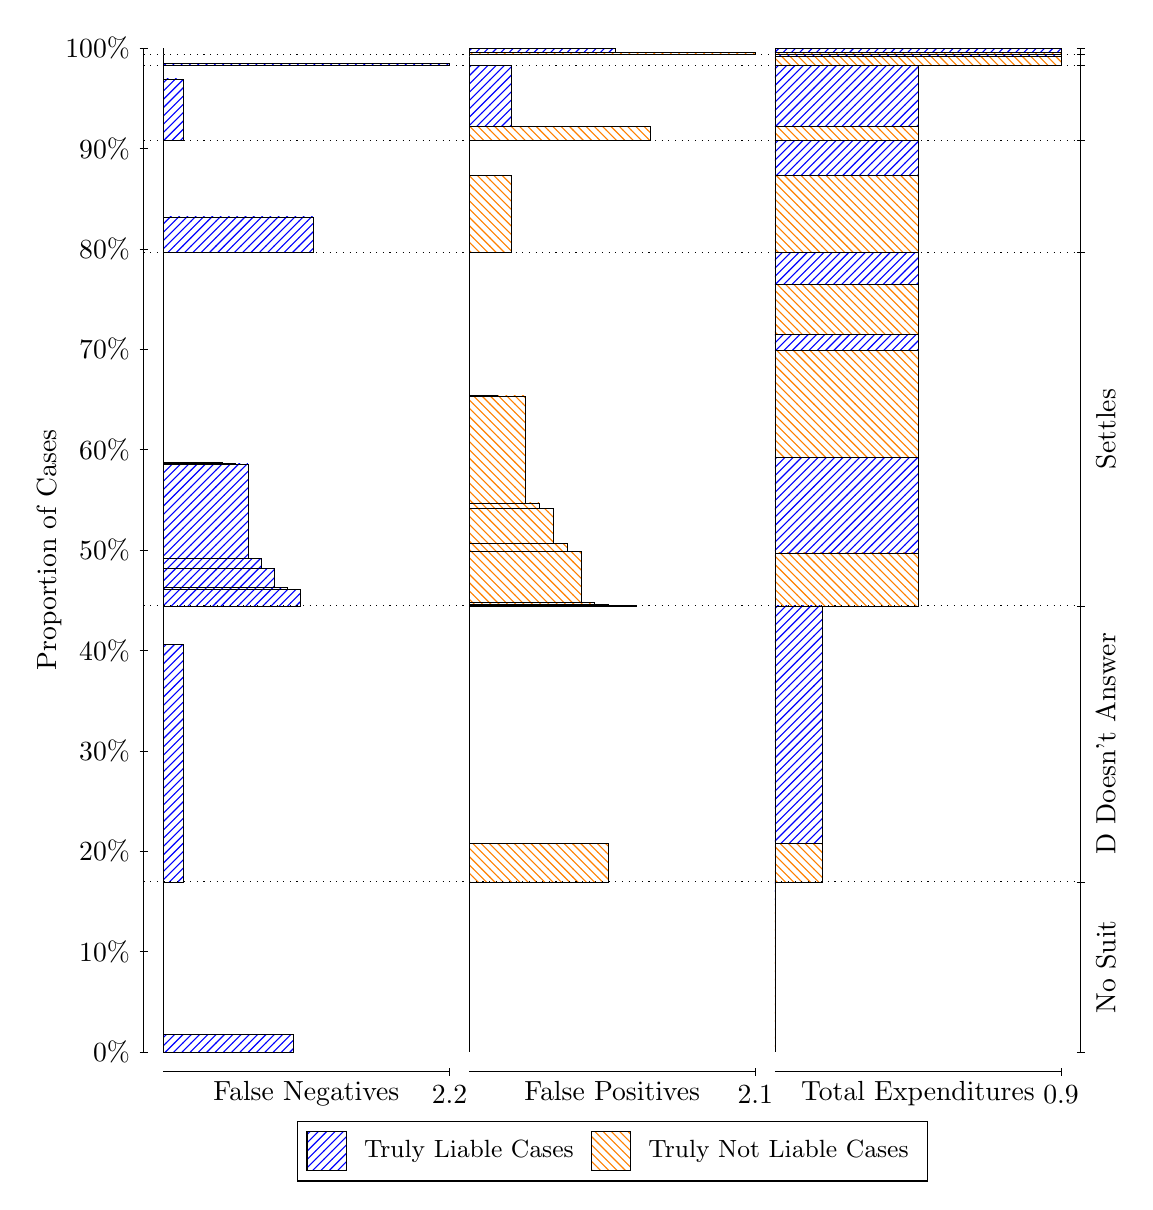
\begin{tikzpicture}
\draw[black, very thin] (1.5,1.75) -- (1.5,14.5);
\node[rotate=90, anchor=center] at (0.3, 8.125) {Proportion of Cases};
\draw[black, very thin] (1.45,1.75) -- (1.55,1.75);
\node[anchor=east] at (1.45, 1.75) {0\%};
\draw[black, very thin] (1.45,3.025) -- (1.55,3.025);
\node[anchor=east] at (1.45, 3.025) {10\%};
\draw[black, very thin] (1.45,4.3) -- (1.55,4.3);
\node[anchor=east] at (1.45, 4.3) {20\%};
\draw[black, very thin] (1.45,5.575) -- (1.55,5.575);
\node[anchor=east] at (1.45, 5.575) {30\%};
\draw[black, very thin] (1.45,6.85) -- (1.55,6.85);
\node[anchor=east] at (1.45, 6.85) {40\%};
\draw[black, very thin] (1.45,8.125) -- (1.55,8.125);
\node[anchor=east] at (1.45, 8.125) {50\%};
\draw[black, very thin] (1.45,9.4) -- (1.55,9.4);
\node[anchor=east] at (1.45, 9.4) {60\%};
\draw[black, very thin] (1.45,10.675) -- (1.55,10.675);
\node[anchor=east] at (1.45, 10.675) {70\%};
\draw[black, very thin] (1.45,11.95) -- (1.55,11.95);
\node[anchor=east] at (1.45, 11.95) {80\%};
\draw[black, very thin] (1.45,13.225) -- (1.55,13.225);
\node[anchor=east] at (1.45, 13.225) {90\%};
\draw[black, very thin] (1.45,14.5) -- (1.55,14.5);
\node[anchor=east] at (1.45, 14.5) {100\%};

\draw[black, very thin] (13.4,1.75) -- (13.4,14.5);
\draw[black, very thin] (13.35,1.75) -- (13.45,1.75);
\node[anchor=west] at (13.35, 1.75) {};
\draw[black, very thin] (13.35,3.9097) -- (13.45,3.9097);
\node[anchor=west] at (13.35, 3.9097) {};
\draw[black, very thin] (13.35,7.4163) -- (13.45,7.4163);
\node[anchor=west] at (13.35, 7.4163) {};
\draw[black, very thin] (13.35,11.907) -- (13.45,11.907);
\node[anchor=west] at (13.35, 11.907) {};
\draw[black, very thin] (13.35,13.33) -- (13.45,13.33);
\node[anchor=west] at (13.35, 13.33) {};
\draw[black, very thin] (13.35,14.282) -- (13.45,14.282);
\node[anchor=west] at (13.35, 14.282) {};
\draw[black, very thin] (13.35,14.42) -- (13.45,14.42);
\node[anchor=west] at (13.35, 14.42) {};
\draw[black, very thin] (13.35,14.5) -- (13.45,14.5);
\node[anchor=west] at (13.35, 14.5) {};

\draw[black, very thin, pattern color=blue, pattern=north east lines] (1.75,1.75) rectangle (3.4015,1.9772);
\draw[black, very thin, pattern color=orange, pattern=north west lines] (1.75,1.9772) rectangle (1.75,3.9097);
\draw[black, very thin, pattern color=blue, pattern=north east lines] (1.75,3.9097) rectangle (1.9977,6.9262);
\draw[black, very thin, pattern color=orange, pattern=north west lines] (1.75,6.9262) rectangle (1.75,7.4163);
\draw[black, very thin, pattern color=blue, pattern=north east lines] (1.75,7.4163) rectangle (3.4841,7.6205);
\draw[black, very thin, pattern color=blue, pattern=north east lines] (1.75,7.6205) rectangle (3.3189,7.648);
\draw[black, very thin, pattern color=blue, pattern=north east lines] (1.75,7.648) rectangle (3.1538,7.8876);
\draw[black, very thin, pattern color=blue, pattern=north east lines] (1.75,7.8876) rectangle (2.9886,8.0176);
\draw[black, very thin, pattern color=blue, pattern=north east lines] (1.75,8.0176) rectangle (2.8235,9.2182);
\draw[black, very thin, pattern color=blue, pattern=north east lines] (1.75,9.2182) rectangle (2.6583,9.2287);
\draw[black, very thin, pattern color=blue, pattern=north east lines] (1.75,9.2287) rectangle (2.4932,9.2387);
\draw[black, very thin, pattern color=blue, pattern=north east lines] (1.75,9.2387) rectangle (2.328,9.2392);
\draw[black, very thin, pattern color=blue, pattern=north east lines] (1.75,9.2392) rectangle (2.1629,9.2409);
\draw[black, very thin, pattern color=orange, pattern=north west lines] (1.75,9.2409) rectangle (1.75,11.907);
\draw[black, very thin, pattern color=blue, pattern=north east lines] (1.75,11.907) rectangle (3.6492,12.356);
\draw[black, very thin, pattern color=orange, pattern=north west lines] (1.75,12.356) rectangle (1.75,13.33);
\draw[black, very thin, pattern color=blue, pattern=north east lines] (1.75,13.33) rectangle (1.9977,14.107);
\draw[black, very thin, pattern color=orange, pattern=north west lines] (1.75,14.107) rectangle (1.75,14.282);
\draw[black, very thin, pattern color=blue, pattern=north east lines] (1.75,14.282) rectangle (5.3833,14.309);
\draw[black, very thin, pattern color=orange, pattern=north west lines] (1.75,14.309) rectangle (1.75,14.42);
\draw[black, very thin, pattern color=orange, pattern=north west lines] (1.75,14.42) rectangle (1.75,14.448);
\draw[black, very thin, pattern color=blue, pattern=north east lines] (1.75,14.448) rectangle (1.75,14.5);
\draw[black, very thin, pattern color=orange, pattern=north west lines] (5.6333,1.75) rectangle (5.6333,3.6825);
\draw[black, very thin, pattern color=blue, pattern=north east lines] (5.6333,3.6825) rectangle (5.6333,3.9097);
\draw[black, very thin, pattern color=orange, pattern=north west lines] (5.6333,3.9097) rectangle (7.4057,4.3998);
\draw[black, very thin, pattern color=blue, pattern=north east lines] (5.6333,4.3998) rectangle (5.6333,7.4163);
\draw[black, very thin, pattern color=orange, pattern=north west lines] (5.6333,7.4163) rectangle (7.7602,7.4178);
\draw[black, very thin, pattern color=orange, pattern=north west lines] (5.6333,7.4178) rectangle (7.5829,7.4188);
\draw[black, very thin, pattern color=orange, pattern=north west lines] (5.6333,7.4188) rectangle (7.4057,7.4362);
\draw[black, very thin, pattern color=orange, pattern=north west lines] (5.6333,7.4362) rectangle (7.2285,7.4549);
\draw[black, very thin, pattern color=orange, pattern=north west lines] (5.6333,7.4549) rectangle (7.0512,8.1073);
\draw[black, very thin, pattern color=orange, pattern=north west lines] (5.6333,8.1073) rectangle (6.874,8.2079);
\draw[black, very thin, pattern color=orange, pattern=north west lines] (5.6333,8.2079) rectangle (6.6967,8.6543);
\draw[black, very thin, pattern color=orange, pattern=north west lines] (5.6333,8.6543) rectangle (6.5195,8.7233);
\draw[black, very thin, pattern color=orange, pattern=north west lines] (5.6333,8.7233) rectangle (6.3423,10.083);
\draw[black, very thin, pattern color=blue, pattern=north east lines] (5.6333,10.083) rectangle (5.9878,10.084);
\draw[black, very thin, pattern color=blue, pattern=north east lines] (5.6333,10.084) rectangle (5.8106,10.085);
\draw[black, very thin, pattern color=blue, pattern=north east lines] (5.6333,10.085) rectangle (5.6333,11.907);
\draw[black, very thin, pattern color=orange, pattern=north west lines] (5.6333,11.907) rectangle (6.165,12.88);
\draw[black, very thin, pattern color=blue, pattern=north east lines] (5.6333,12.88) rectangle (5.6333,13.33);
\draw[black, very thin, pattern color=orange, pattern=north west lines] (5.6333,13.33) rectangle (7.9374,13.504);
\draw[black, very thin, pattern color=blue, pattern=north east lines] (5.6333,13.504) rectangle (6.165,14.282);
\draw[black, very thin, pattern color=orange, pattern=north west lines] (5.6333,14.282) rectangle (5.6333,14.393);
\draw[black, very thin, pattern color=blue, pattern=north east lines] (5.6333,14.393) rectangle (5.6333,14.42);
\draw[black, very thin, pattern color=orange, pattern=north west lines] (5.6333,14.42) rectangle (9.2667,14.448);
\draw[black, very thin, pattern color=blue, pattern=north east lines] (5.6333,14.448) rectangle (7.4943,14.5);
\draw[black, very thin, pattern color=orange, pattern=north west lines] (9.5167,1.75) rectangle (9.5167,3.6825);
\draw[black, very thin, pattern color=blue, pattern=north east lines] (9.5167,3.6825) rectangle (9.5167,3.9097);
\draw[black, very thin, pattern color=orange, pattern=north west lines] (9.5167,3.9097) rectangle (10.122,4.3998);
\draw[black, very thin, pattern color=blue, pattern=north east lines] (9.5167,4.3998) rectangle (10.122,7.4163);
\draw[black, very thin, pattern color=orange, pattern=north west lines] (9.5167,7.4163) rectangle (11.333,8.0871);
\draw[black, very thin, pattern color=blue, pattern=north east lines] (9.5167,8.0871) rectangle (11.333,9.2982);
\draw[black, very thin, pattern color=orange, pattern=north west lines] (9.5167,9.2982) rectangle (11.333,10.658);
\draw[black, very thin, pattern color=blue, pattern=north east lines] (9.5167,10.658) rectangle (11.333,10.862);
\draw[black, very thin, pattern color=orange, pattern=north west lines] (9.5167,10.862) rectangle (11.333,11.498);
\draw[black, very thin, pattern color=blue, pattern=north east lines] (9.5167,11.498) rectangle (11.333,11.907);
\draw[black, very thin, pattern color=orange, pattern=north west lines] (9.5167,11.907) rectangle (11.333,12.88);
\draw[black, very thin, pattern color=blue, pattern=north east lines] (9.5167,12.88) rectangle (11.333,13.33);
\draw[black, very thin, pattern color=orange, pattern=north west lines] (9.5167,13.33) rectangle (11.333,13.504);
\draw[black, very thin, pattern color=blue, pattern=north east lines] (9.5167,13.504) rectangle (11.333,14.282);
\draw[black, very thin, pattern color=orange, pattern=north west lines] (9.5167,14.282) rectangle (13.15,14.393);
\draw[black, very thin, pattern color=blue, pattern=north east lines] (9.5167,14.393) rectangle (13.15,14.42);
\draw[black, very thin, pattern color=orange, pattern=north west lines] (9.5167,14.42) rectangle (13.15,14.448);
\draw[black, very thin, pattern color=blue, pattern=north east lines] (9.5167,14.448) rectangle (13.15,14.5);
\draw[black, dotted] (1.5,3.9097) -- (13.4,3.9097);
\draw[black, dotted] (1.5,7.4163) -- (13.4,7.4163);
\draw[black, dotted] (1.5,11.907) -- (13.4,11.907);
\draw[black, dotted] (1.5,13.33) -- (13.4,13.33);
\draw[black, dotted] (1.5,14.282) -- (13.4,14.282);
\draw[black, dotted] (1.5,14.42) -- (13.4,14.42);
\draw[black, very thin] (1.75,1.5) -- (5.3833,1.5);
\node[anchor=north] at (3.5667, 1.5) {False Negatives};
\draw[black, very thin] (5.3833,1.45) -- (5.3833,1.55);
\node[anchor=north] at (5.3833, 1.45) {2.2};

\draw[black, very thin] (5.6333,1.5) -- (9.2667,1.5);
\node[anchor=north] at (7.45, 1.5) {False Positives};
\draw[black, very thin] (9.2667,1.45) -- (9.2667,1.55);
\node[anchor=north] at (9.2667, 1.45) {2.1};

\draw[black, very thin] (9.5167,1.5) -- (13.15,1.5);
\node[anchor=north] at (11.333, 1.5) {Total Expenditures};
\draw[black, very thin] (13.15,1.45) -- (13.15,1.55);
\node[anchor=north] at (13.15, 1.45) {0.9};

\node[black, centered, rotate=90] at (13.72, 2.8298) {No Suit};
\node[black, centered, rotate=90] at (13.72, 5.663) {D Doesn't Answer};
\node[black, centered, rotate=90] at (13.72, 9.6618) {Settles};





\draw (7.449999999999999,1.5) node[draw=none] (baseCoordinate) {};
\begin{scope}[align=center]
        \matrix[scale=0.5, draw=black, below=0.5cm of baseCoordinate, nodes={draw}, column sep=0.1cm]{
            \node[rectangle, draw, minimum width=0.5cm, minimum height=0.5cm, pattern=north east lines, pattern color=blue] {}; &
            \node[draw=none, font=\small] (B) {Truly Liable Cases}; &
            \node[rectangle, draw, minimum width=0.5cm, minimum height=0.5cm, pattern=north west lines, pattern color=orange] {}; &
            \node[draw=none, font=\small] (B) {Truly Not Liable Cases}; \\
            };
\end{scope}

\end{tikzpicture}
\end{document}